% !TeX root = ../../ZF_bmicha_Ana.tex
\subsection{Schwerpunkte \texorpdfstring{\hfill S.76}{S.76}}\vspace{3pt}

    \subsubsection{2D}
    $\sigma(x,y)$: Flächendichte $[kg/m^2 ] $
        \begin{align*}
            &m = \iint \sigma(x,y) \, dA\\[0.25em]
            x_s =&\, \frac{1}{m} \iint x \cdot \sigma(x,y) \, dA\\
            y_s =&\, \frac{1}{m} \iint y \cdot \sigma(x,y) \, dA
        \end{align*}
    \textit{Keine Angabe für $\sigma$: $\sigma = 1$}
    \vspace{5pt}
    \subsubsubsection{Schwerpunkt eines Kreisausschnitts}
    \begin{minipage}{0.49\linewidth}
        \begin{align*}
        x_s &= 0 \\
        y_s &= \frac{2r^2 sin \alpha}{b} = r \frac{l}{b}
        \end{align*}
    \end{minipage}
    \begin{minipage}{0.49\linewidth}
        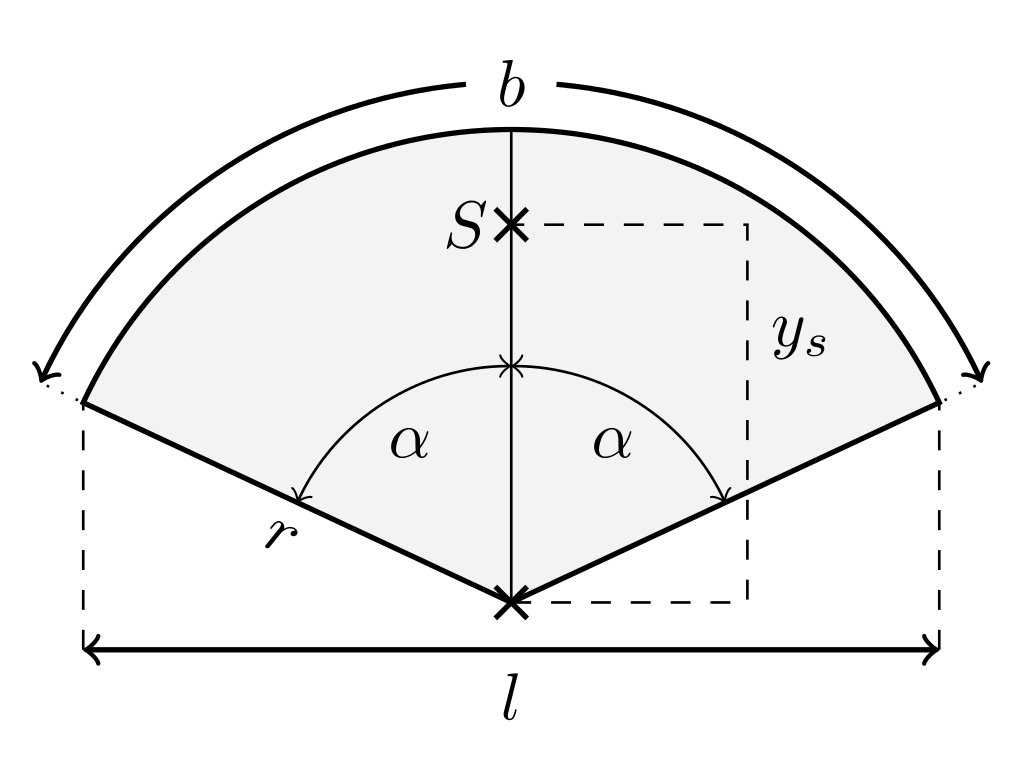
\includegraphics[width=0.95\linewidth]{src/Mehrdimensionale-Funktionen_Integralrechnung/1024px-Circular-sector-centroid.svg.png}
    \end{minipage}
    
    \subsubsubsection{Schwerpunkt eines Kreissegments}
    
    \begin{minipage}{0.49\linewidth}
        \begin{align*}
        x_s &= 0 \\
        y_s &= \frac{s^3}{12 A} - r\cdot \cos{\frac{\alpha}{2}}\\ 
        A &= \frac{r^2}{2} \cdot \left( \frac{\pi \cdot \alpha}{180}- \alpha \right)\\
        \left[  \alpha \right] &= \textrm{Grad}
        \end{align*}
    \end{minipage}
    \begin{minipage}{0.49\linewidth}
        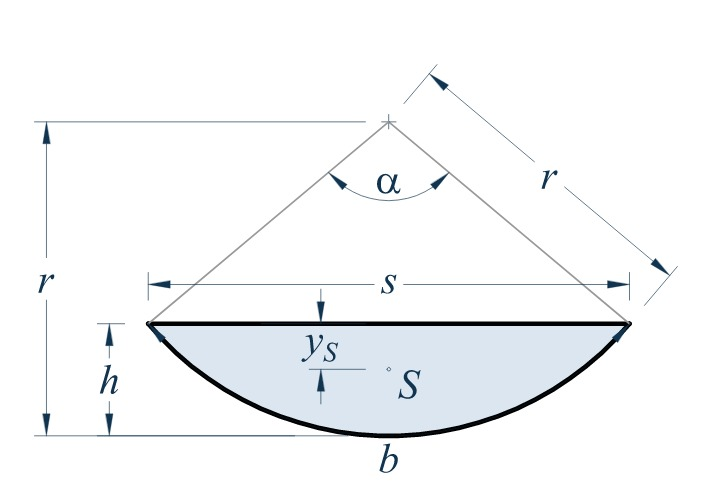
\includegraphics[width = \linewidth]{src/Mehrdimensionale-Funktionen_Integralrechnung/Kreissegment.jpeg}
    \end{minipage}
    
    \subsubsection{Zusammengesetzter Schwerpunkt}
    $$ x_s = \frac{1}{A_{ges}} \cdot \left( A_1 \cdot \Delta x_{s1} \pm A_2 \cdot \Delta x_{s2} \pm \dots \right) $$
    
    \subsubsection{3D}
    $\rho(x,y,z)$: Volumendichte $[kg/m^3 ] $
        \begin{align*}
            &m = \iiint \rho(x,y,z) \, dV\\[0.25em]
            x_s =&\, \frac{1}{m} \iiint x \cdot \rho(x,y,z) \, dV\\
            % y_s =&\, \frac{1}{m} \iiint y \cdot \rho(x,y,z) \, dV
            y_s =&\, \dots
        \end{align*}
        \vspace{-0.45em}
    \textit{Keine Angabe für $\rho$: $\rho = 1$}
    \vspace{0.5em}
    
    \cbreak
        

        